
\documentclass[11pt]{beamer}

\usetheme{Warsaw}
\usepackage{mathrsfs}
\usepackage{amsmath}
\usepackage{graphicx}
\usepackage{caption}
%\usepackage{subcaption}

%Mathematical writting
\theoremstyle{plain}
\newtheorem{thm}{Theorem}[section]

\theoremstyle{definition}
\newtheorem{dfn}{}[section]

%New commands
\newcommand\ChangeFont{\fontsize{9}{7.2}\selectfont}
\newcommand{\y}{\textbf{y}}
\newcommand{\x}{\textbf{x}}

\newcommand{\p}{\mathbb{P}}
\newcommand{\like}{\p_{like}}
\newcommand{\prior}{\p_{prior}}
\newcommand{\post}{\p_{post}}

\begin{document}
%Presentation slide

\begin{frame}{CFD Group}
\begin{center}
\large{Simon Fraser University}
\end{center}
\begin{figure}
\includegraphics[scale=0.15]{log}
\end{figure}
\begin{center}
Parameter Estimation Using Gaussian Process Regression.
\end{center}

\begin{center}
Juan Gabriel Garc{\'i}a
\end{center}

\begin{center}
February 20 of 2017
\end{center}
\end{frame}

\AtBeginSection[] 
{ 
\begin{frame} 
\ChangeFont 
\frametitle{Content} 
\tableofcontents[currentsection] 
\end{frame} 
} 




\section{Problem of Interest}

\begin{frame}{Problem of Interest}

\begin{columns}[c]
\column{1.5in}
Consider the model of pollutant transport
\begin{equation*}
\partial_{t} c+L(\theta)c=\sum_{k}q_{k}
\end{equation*}
Goal: Estimate $q_{i}$ and $\theta$ using the measurements $R_{j}$.
\column{1.5in}
\begin{figure}
\includegraphics[scale=0.36]{BCtrail}
\ChangeFont
\caption{Taken from: Hosseini, Stockie. A finite volume scheme....}
\end{figure}

\end{columns}
\end{frame}

\section{Explaining the Basics}

\begin{frame}
\frametitle{Toy Problem}
\begin{dfn}
\begin{equation}\label{eqnPDE}
\left\{
        \begin{array}{ll}
                \Delta u=\exp(-b\|x\|) & x\in \Omega=[0,1]\times [0,1] \\
                u=0 & x\in\partial\Omega
        \end{array}
\right.
\end{equation}
\end{dfn}
\begin{itemize}
\item The function $u$ is a mathematical approximation for a function 
$\tilde{u}$ with physical meaning. 
\item The behavior of $\tilde{u}$ is modeled by equation ($\ref{eqnPDE}$).
\item We want to estimate the value of $b$ that explains experimental
measurements of $\tilde{u}$.
\end{itemize}
\end{frame}

\begin{frame}
\frametitle{`Experimental' Setting}
\begin{figure}
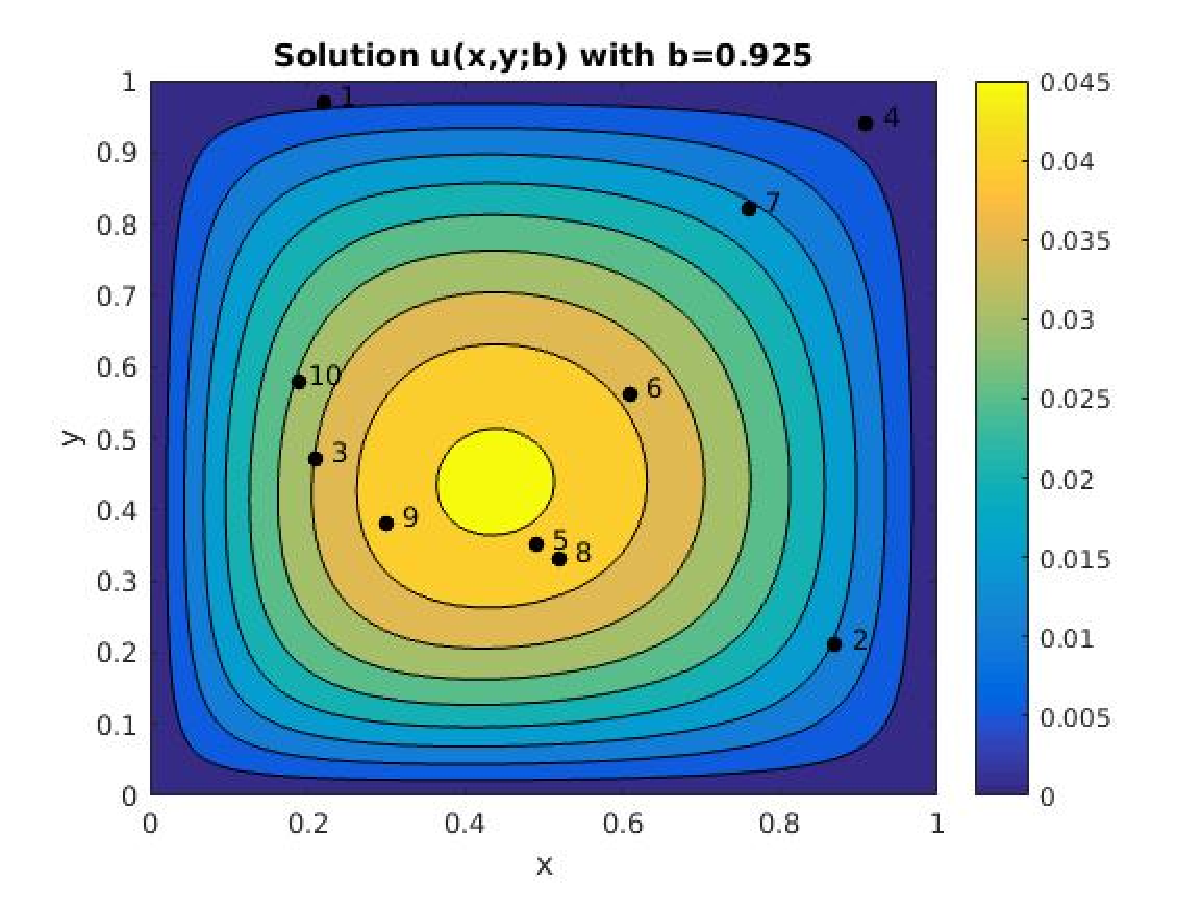
\includegraphics[scale=0.4]{solu}
\caption{Location where the measurements 
$\textbf{y}:=(\tilde{u}(\x_{1};b),\ldots,\tilde{u}(\x_{10};b))$ were obtained}
\end{figure}
\end{frame}


\begin{frame}
\frametitle{How to Find the Value of  $b$ that Explains $\y$}
\begin{itemize}
\item We can simulate only for an small number of values of $b$.
\item We need to interpolate for the values of $b$ we cannot simulate.
\end{itemize}
\begin{dfn} 
A Gaussian process (GP) is a collection of random variables $\{g(x)\}_{x\in A}$, for some set $A$,
possibly uncountable,
 such that any finite subset of random variables
 $\{g(x_{k})\}_{k=1}^{N}\subset\{g(x)\}_{x\in A}$ for
$\{x_{k}\}_{k=1}^{N}\subset A$ are jointly Gaussian.
\end{dfn}
\end{frame}

\begin{frame}
\frametitle{Multivariate Gaussian Distribution}
\begin{dfn}
Two random vector $X\in\mathbb{R}^{n}$ and $Y\in\mathbb{R}^{m}$
are jointly Gaussian if their joint density function is given by
\begin{equation*}
\frac{1}{(2\pi)^{\frac{m+n}{2}}|\Sigma|^{\frac{1}{2}}}
\exp(-([x,y]-[\mu_{x},\mu_{y}])
\underbrace{\begin{bmatrix}
\Sigma_{xx} & \Sigma_{xy}\\
\Sigma_{xy}^{T} & \Sigma_{yy}
\end{bmatrix}}_{\Sigma}
([x,y]-\underbrace{[\mu_{x},\mu_{y}]}_{\mu})^{T})
\end{equation*}
%In this case we write
%\begin{equation*}
%(X,Y)\sim\mathcal{N}(\mu,\Sigma)
%\end{equation*}
\end{dfn}
\begin{itemize}
\item Marginal distribution is multivariate Gaussian.
	\begin{itemize}
		\item $X\sim\mathcal{N}(\mu_{x},\Sigma_{xx})$.
		\item $Y\sim\mathcal{N}(\mu_{y},\Sigma_{yy})$.
	\end{itemize}
\item Conditional distribution is multivariate Gaussian.
	\begin{itemize}
		\item $X|Y=y\sim\mathcal{N}(\mu_{x}-\Sigma_{xy}\Sigma_{yy}^{-1}
		(y-\mu_{y}),\Sigma_{xx}-\Sigma_{xy}\Sigma_{yy}^{-1}\Sigma_{yx})$.
	\end{itemize}
\end{itemize}
\end{frame}


\begin{frame}
\frametitle{Relating $b$ and $u$}
\begin{figure}
\includegraphics[scale=0.4]{fitted}
\end{figure}
\end{frame}

%%%%%%%%%%%%%%%%%%%%%%%%%%%%%%%5



%%%%%%%%%%%%%%%%%%%%%%%%%

\begin{frame}
\frametitle{Finding $b$}
\begin{dfn}
Having a vector $\y$ of measurements of $\tilde{u}$  we can relate them with
the GP regression $G$ via
\begin{equation*}
\y=G(b)+\epsilon \qquad \epsilon\sim\mathcal{N}(0,5.4\times 10^{-3}).
\end{equation*}
We can estimate  $b$ given the experimental data $\textbf{y}$
 using $\textit{Bayes rule}$
\begin{equation*}
\post(b|\y)\propto \like(\y|b)\prior(b).
\end{equation*}
with
\begin{equation*}
\y|b\sim \mathcal{N}(G(b),\underbrace{5.4\times 10^{-3}}_{\lambda^{2}}), \qquad b\sim U(0,2)
\end{equation*}
\end{dfn}
\end{frame}

\begin{frame}
\frametitle{Distributions}
\begin{columns}[c]
\column{1.5 in}
\begin{figure}
\includegraphics[scale=0.32]{prior_posterior}
\end{figure}

\column{1.3in}

\begin{eqnarray*}
\post(b|\y)\propto\like(\y|b)\prior(b)\\
\propto \textbf{1}_{(0,2]}(b)e^{-\frac{1}{2\lambda^{2}}\|G(b)-\textbf{y}\|_{2}^{2}}
\end{eqnarray*}
\end{columns}
\end{frame}

\begin{frame}
\frametitle{Why is Useful to Find the Posterior?}
\begin{itemize}
\item To find central tendency measures.
\begin{eqnarray*}
b_{MAP}=argmax_{b}\quad\post(b|\textbf{y}). 
\qquad\text{(Maximum a posteriori)}\\
b_{CM}=\int_{\mathbb{R}}b\post(b|\textbf{y})db.
\qquad\text{(Conditional mean)}. \\
\end{eqnarray*}
\item Assess the uncertainty in the estimation
\begin{equation*}
\int_{\mathbb{R}}(b-b_{cm})^{2}\post(b|\textbf{y})db.
\end{equation*}
\end{itemize}
\end{frame}

\begin{frame}
\frametitle{Sampling from a Probability Distribution}

\begin{columns}[c]
\column{1.1in}
\begin{figure}
\includegraphics[scale=0.25]{histogram_mcmc}
\end{figure}

\column{2.0in}
\ChangeFont
Metropolis Hastings Algorithm
\begin{enumerate}
\item pick a point $q_{1}$\\
\textbf{for} j=2:N
\item $\qquad$Draw $u\sim U([0,\alpha])$
\item $\qquad q_{j}\leftarrow q_{j-1}+u$
\item $\qquad$Compute $\post(q_{j}|\textbf{y})$
\item $\qquad\beta\leftarrow\min(1,\frac{\post(q_{j}|\textbf{y})}{\post(q_{j-1}|\textbf{y})})$
\item $\qquad$Draw $w\sim U([0,1])$\\
%\\
$\qquad\qquad\qquad$\textbf{if} $w<\beta$
\item $\qquad\qquad q_{j-1}=q_{j}$\qquad(Accept move)\\
%\\
$\qquad\qquad$\textbf{else}
\item
        $\qquad\qquad q_{j-1}=q_{j-1}$\\
\textbf{end}\\
\textbf{end}
\end{enumerate}
\end{columns}
\end{frame}

\begin{frame}
\frametitle{Obtaining Statistics}
By the strong law of large numbers
\begin{equation*}
b_{cm}=\int_{(0,2]}b\post(b|D)db\approx\frac{1}{5000}
\sum_{j=1}^{5000}b_{j}=0.9247042.
\end{equation*}
\begin{equation*}
\int_{(0,2]}(b-b_{cm})^{2}\post(b|D)db\approx\frac{1}{5000}\sum_{j=1}^{5000}(b_{j}-b_{cm})^{2}=0.01427.
\end{equation*}
With $95\%$ percent of confidence
\begin{equation*}
b\in [0.68579,1.16361].
\end{equation*}
\end{frame}

%%%%%%%%%%%%%%%%%%%%%%%%%%%%%%%%%%%%%%%%%%%%%%%%%Presentation 3 %%%%%%%%%%%%%%%%%%%%%%%%%%%
\section{Application to Pollutant Dispersion Model}
\begin{frame}{Problem of Interest}

\begin{columns}[c]
\column{1.5in}
Consider the model of pollutant transport
\begin{equation*}
\partial_{t} c+L(\theta)c=\sum_{k}q_{k}
\end{equation*}
Goal: Estimate $q_{i}$ and $\theta$ using the measurements $R_{j}$.
\column{1.5in}
\begin{figure}
\includegraphics[scale=0.36]{BCtrail}
\ChangeFont
\caption{Taken from: Hosseini, Stockie. A finite volume scheme....}
\end{figure}

\end{columns}
\end{frame}

\begin{frame}
\frametitle{Mathematical Model}
\begin{equation*}
\partial_{t} c(\textbf{x},t)+\nabla\cdot(\textbf{u}(\textbf{x},t)c+\textbf{S}(\textbf{x},t)\nabla c)
=q(\textbf{x},t)\qquad\text{on }\mathbb{R}^{2}\times\mathbb{R}_{\geq 0}\times(0,T).
\end{equation*}
\begin{itemize}
\item $\textbf{u}(\textbf{x},t)=(u_{x}(z,t),u_{y}(z,t),u_{set})$ 
(Wind velocity field)
\item $\|(u_{x},u_{y})\|_{2}\propto\left(\frac{z}{z_{r}}\right)^{\gamma}$.
\item $\textbf{S}=diag(s_{x},s_{y},s_{z})$ (Eddy diffusion matrix)
\item $s_{z}=f(L,z_{cut})$, where $\frac{1}{L}=a+b\log_{10}(z_{0})$.
\item $s_{x}=s_{y}=g(z_{i},L)$, with $z_{i}$ Mixing layer height.
\end{itemize}
\end{frame}

\begin{frame}
\frametitle{Are all the Parameters Relevant?}
\ChangeFont
To assess the relevance of the parameters we do a Sensitivity analysis.
\begin{itemize}
\item Given a function of interest $\varphi$ we decompose it as 
\begin{equation*}
\varphi(x_{1},\ldots,x_{n})=\varphi_{0}+\sum_{k=1}^{n}\varphi_{k}(x_{k})+
\sum_{1\leq k< l\leq n}\varphi_{kl}(x_{k},x_{l})+\ldots+
\varphi_{1,2,\ldots,n}(x_{1},\ldots,x_{n}).
\end{equation*}
\item With the constraint
\begin{equation}\label{eqnSobolCond1}
\int_{[0,1]}\varphi_{i_{1},\ldots,i_{j}}dx_{i_{k}}=0\qquad\text{if }  i_{k}\in \{i_{1},\ldots,i_{j}\}
\end{equation}
\item This condition allows to find each element in the decomposition recursively.
\end{itemize}
\end{frame}

\begin{frame}
\frametitle{Sobol Indices}
The total variance $D$ of $\varphi$ is defined as
\ChangeFont
\begin{equation*}
D=\int_{\Omega^{n}}\varphi^{2}(x)dx-\varphi_{0}^{2}.
\end{equation*}
Similarly we can compute the partial variances as
\begin{equation*}
D_{i_{1},\ldots,i_{s}}=\int_{[0,1]^{n-1}}\varphi^{2}_{i_{1},\ldots,i_{s}}dx_{i_{1}}\ldots dx_{i_{s}}.
\end{equation*}
With these variances we define the $s-th$ order  Sobol index
\begin{equation*} 
S_{i_{1},\ldots,i_{s}}=\frac{D_{i_{1},\ldots,i_{s}}}{D}.
\end{equation*}
To measure the relevance of the $i$-th parameter we calculate
\begin{equation*}
S_{i}+S_{i1}+S_{i2}+\ldots+S_{i12}+S_{i13}+\ldots+S_{12\ldots,i,\ldots, n}.
\text{ (Total Sobol Index)}
\end{equation*}
\end{frame}







\begin{frame}
\frametitle{Sensitivity Analysis}
\begin{columns}[c]
\column{1.5in}
\ChangeFont
For the problem we have the following parameters
\begin{itemize}
\item $\gamma$: Fitting parameter for the z dependence of the velocity.
\item $z_{0}$: Roughness length.
\item $z_{i}$: Mixing layer height.
\item $L$: Monin-Obukhov length.
\item $z_{cut}$: cutoff height.
\end{itemize}

By using the packages Sensitivity and DiceKringing we estimate the Sobol indices 
for each on of the variables in each one of the measurement sites. 
\column{1.5in}
\begin{figure}
\includegraphics[scale=0.3]{full_sensitivity}
\end{figure}

\end{columns}
\end{frame}



\begin{frame}
\frametitle{What About the Sources?}

\begin{dfn}
The deposition behaves linearly  with respect to the values of the 4  sources,
hence
\begin{equation*}
\begin{bmatrix}
R_{1} \\
R_{2} \\
\vdots\\
R_{9}
\end{bmatrix}=A(\gamma,z_{0},L)
\begin{bmatrix}
q_{1}\\
\vdots\\
q_{4}
\end{bmatrix}
+\vec{\epsilon},\qquad\text{ where } \vec{\epsilon}\sim\mathcal{N}(0,
\sigma^{2}I_{9\times 9}).
\end{equation*}
To evaluate the matrix $A(\gamma,z_{0},L)$ in points $(\gamma,z_{0},L)$ outside the experimental design we fit a 
Gaussian process in each of the 36 entries of $A(\gamma,z_{0},L)$.
\end{dfn}
\end{frame}

\begin{frame}
\frametitle{Design of the experiment}
\begin{columns}[c]
\column{1.5in}
\begin{itemize}
\item We proceed to do an space filling design in the $(\gamma,z_{0},L)$-plane.
\item We do a MaxiMin design on 64 points, to achieve the optimization we use a particle swarm 
algorithm.
\end{itemize}
\column{1.5in}
\begin{figure}
\includegraphics[scale=0.3]{desing64}
\end{figure}
\end{columns}
\end{frame}
\begin{frame}
\frametitle{Simulations}
\ChangeFont
\begin{columns}[c]
\column{1.5in}
\begin{itemize}
\item On the experimental design, Bamdad ran the finite volume code on a 
$30\times 30$ grid on the square $\Omega=[-200m,1200 m]^{2}$. 

\item The idea is to run the code $4$ times, each time setting on of the sources
with an emission of $1$ and $0$ the other $3$.
\end{itemize}

\column{1.5in}
\begin{figure}
\includegraphics[scale=0.3]{deposition}
\end{figure}


\end{columns}

\end{frame}



\begin{frame}
\frametitle{Probabilistic Model}

\begin{dfn}
Our goal is to estimate the values of $p:=(\gamma,z_{0},L)$ and 
$q:=(q_{1},q_{2},q_{3},q_{4})$ given the measurements
$\vec{R}$. Mathematically we want to estimate:

\begin{equation*}
\post(p,q|\vec{R})\propto
\underbrace{\like(\vec{R}|p,q)\prior(p)\prior(q)}_{\text{Assuming $p$ and $q$ independent}}
\end{equation*}
We assume $p\sim Uniform$ over the domain of definition of the parameters.
 
\end{dfn}
\end{frame}

\begin{frame}
\frametitle{What about $q$?}
To set a prior for $q$ we first need to check what do we know about $q$. This knowledge can be 
summarized as follows
\begin{itemize}
\item $q_{k}>0$ for $k=1,2,3,4$.
\item If we trust the engineers the most likely value for $q$ is the engineers estimate.
\item If we think they know what they are doing the true value for $q$ cannot be very far away from their
estimate.
\end{itemize}
\end{frame}

\begin{frame}
\frametitle{Choosing a prior for $q$}
\begin{columns}[c]
\column{2.2in}
A consistent assumption is $q_{k}\sim Ga(\alpha_{k},\beta_{k})$,for $k=1,2,3,4$,
the following conditions that define $\alpha_{k}$ and $\beta_{k}$ for all $k$ uniquely.

\begin{itemize}
\item $\beta_{k}(\alpha_{k}-1)=q_{eng,k}$
\item $qgamma(0.99,\alpha_{k},\beta_{k})=3q_{eng,k}$
\end{itemize}
\column{1.5in}
\begin{figure}
\includegraphics[scale=0.3]{gamma_generic}
\end{figure}
\end{columns}
\end{frame}


\begin{frame}
\frametitle{Getting the posterior}
\begin{itemize}
\item We have $\like(\vec{m}|q,p)\propto
\exp(-\frac{1}{2\sigma_{\epsilon}^{2}}\|m-A(p)q\|^{2}_{2})$
\item Also $\prior(q_{k})\propto q_{k}^{\alpha_{k}-1}\exp(\beta_{k}q_{k})$.
\item and $\prior(p)\propto\textbf{1}_{[0.1,0.4]\times[10^{-3},2]\times[-500,-1]}
:=\textbf{1}_{B}$
\end{itemize}
\bigskip
Then
\newline 
\newline
$\post(q,p|\vec{m})\propto
\textbf{1}_{B}\left(\prod_{k=1}^{4}q_{k}\right)\exp(-\frac{1}{2\sigma_{\epsilon}^{2}}\|\vec{m}-A(p)q\|^{2}_{2}+
\sum_{k=1}^{4}\beta_{k}q_{k})$.
\end{frame}


\begin{frame}
\frametitle{Sampling the Posterior}
Using MH algorithm with step size $0.11$
\begin{columns}[c]
\column{1.5in}
\begin{figure}
\includegraphics[scale=0.3]{mixings}
\end{figure}

\column{1.5in}
\begin{figure}
\includegraphics[scale=0.3]{hists}
\end{figure}
\end{columns}
\end{frame}


\section{What is Next?}
\begin{frame}
\frametitle{What is Next}
\begin{enumerate}
\item What I have done so far:
	\begin{itemize}
	\item Chapter 2 of my Thesis is in second revision.
	\item Chapter 3 of my Thesis is in first revision.
	\end{itemize}

\item What is next:
	\begin{itemize}
	\item Complete/debug my codes.
	\item Organize the results to write a paper with John and Bamdad.
	\item Start to write Chapter 4.
	\item Try to expand the project in the summer.
	\end{itemize}
\end{enumerate}
\end{frame} 














\end{document}
